\section{Reasons for SPI}

Choices fell on SPI. Alternatives before taking the choice were:

\begin{description}
\item[\(GPIO\)] The Panda Board offer multiple pins which can be either controlled with userspace or kernelspace commands. Speed is not determined by official 
instructions but below SPI bus speed.\footnote{\url{https://groups.google.com/forum/\#!msg/pandaboard/mqfaT54NzWk/UH5HIhlg\_TsJ}}
\item[\(I^2C\)] Various pins available. Choice number 2 for the project.
\item[\(Serial Port\)] One connector available but used for debugging. Speed is measured in baud.
\item[\(SPI\)] Multiple pins on both expansion connectors available. Speed successfully tested up to 10 MHz.
\end{description}

Main reason for the group's choice was the speed and the educational effect of appling a SPI implementation to an ARM-Board.

An oscilloscope was used for debugging purpose and was needed multiple times.

\section{SPI for Linux}

The SPI interface is documented in \url{http://www.kernel.org/doc/Documentation/spi/spi-summary}. There was no need for a MISO\footnote{Master In, Slave Out} connection as the LED-bar was solely receiving data.
Different clock modes could be used but as the clock was not used in this project altogether to the expense of inability to drive the LED bar in parallel with other SPI slaves.

Two different approaches for programming were available:
\begin{enumerate}
\item spidev is a development driver which is already included in the kernel. It can be used to test SPI functionality but is not as much configurable as a custom protocol driver.
\item SPI protocol drivers allow the whole range of configuration. Some kernel provided structures have to be used.
\end{enumerate}


ASYNC SYNC MESSAGES

\subsection{Various Howtos}

The instruction for using the GPIO ports for latching were taken from
\url{http://www.nerdenmeister.org/2011/11/13/using-the-gpio-pins-on-a-pandaboard/} in addition to the official kernel documentation.
The link only provides userspace toggling but similar functionality can be archived by using direct kernel functions as pointed out 
by \url{http://www.kernel.org/doc/Documentation/gpio.txt}.

Most useful for this project is the rather lengthly Howto from Scott Ellis available at \url{http://www.jumpnowtek.com/index.php?option=com\_content&view=article&id=57&Itemid=62}. His tutorial covered the whole development process of an SPI protocol driver and was 
written for the Beagleboard. The author of this project adapted it to the Pandaboard and most of the kernel module code is based on the last
version of Scott's driver. We want to thank the author as his documentation was the only complete one.

\section{Practical Work}

For preparation some necessary header files for compiling a kernel module are required. There is no need for a complete kernel source as 
wrongly pointed out by the Beagleboard-group. As the complete sources for the Texas Instrument kernel are not available the headers 
are the only option. 

The installation in a Debian environment is done by \textsl{sudo apt-get linux-headers-omap4}. The files will be available in the 
directory \textsl{/usr/src}.

Compiling is done with a self-made Makefile which is available in the Github repository. Mainly it specified the location for the header files
and inserts the module if the compilation succeeded. Another option for the makefile is to remove the kernel by one command for increasing 
the handling for other group members.

Practical for visualisation of the source code is an activity diagram as shown in figure~\ref{fig:actKernel}. After the critical 
initialisation part which was encountered in error frequently due to insufficient rights for inserting the module or taking bogus parametres
in the development phase the LED-bar is accessible through a char device called \textsl{/dev/embeddedLamp}. It starts running a counter 
which omits the chip programming specialities and just shifts binary ones beginning from zero. When the total amount of bits for the 
LED is reached it starts from zero again.

Every message which is transmitted over the SPI-bus contains five 8 bit unsigned integers, representing each part of the LED-bar. The 
data is wrapped in a C-structure which interface is given by the Linux kernel. Also, the five messages are part of a transfer structure which 
is finally send over SPI.

\begin{figure}[h]
   \centering
   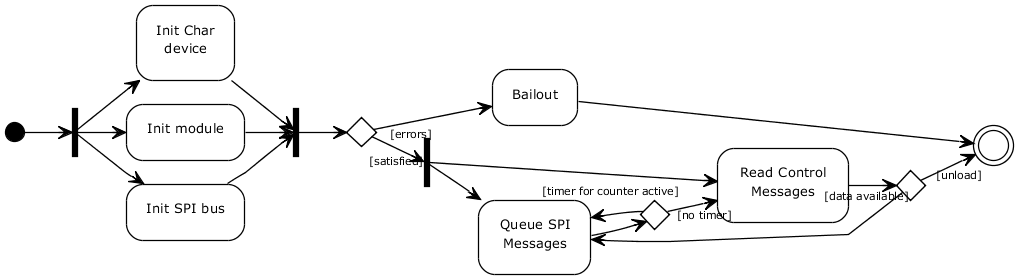
\includegraphics[width=\textwidth]{img/kernel_activity.png}%
   \caption{Activity Diagram for Kernel Module}
   \label{fig:actKernel}%
\end{figure}

One additional interface was included by reading the char device. It displays the total amount of sent counter messages and the amount of 
lost messages. The loss was between 1\% and 0.1\% of total messages, depending and correlating on the bus speed.
An example command would be \textsl{cat /dev/embeddedLamp}.

By sending the command \textsl{start} the counter starts and by sending \textsl{stop} it supposedly should stop. An example command is \textsl{echo 'start' >/dev/embeddedLamp}.

Another way of accessing the LED-bar is by echo'ing the hexadecimal representation to the char device, e.g. \textsl{echo 'DEADBEEF00' >/dev/embeddedLamp}. The kernel driver searches for a ten char long string and lights up the LED. This is exportable for userspace access and was finally used for the WiFi-Quality representation.
